\documentclass[9pt,twocolumn,twoside]{gsajnl}
% Use the documentclass option 'lineno' to view line numbers

\articletype{inv} % article type
% {inv} Investigation 

\title{CaMK (CMK-1) and O-GlcNAc transferase (OGT-1) modulate mechanosensory responding and learning in  \textit{C. elegans}}

\author[$\ast$]{Tiffany A. Timbers}
\author[$\ast$]{Evan L. Ardiel}
\author[$\ast$]{Kirsten C. Y. Lee}
\author[$\S$]{Javad Safaei}
\author[$\dagger$,$\ddagger$]{Steven L. Pelech}
\author[$\ast$]{Troy McDiarmid}
\author[$\ast$,$\ast\ast$,1]{Catharine H. Rankin}

\affil[$\ast$]{Brain Research Centre, University of British Columbia, 2211 Wesbrook Mall, Vancouver, British Columbia, V6T 2B5 Canada}
\affil[$\S$]{Department of Computer Science, University of British Columbia, 2366 Main Mall, Vancouver, British Columbia, V6T 1Z4 Canada}
\affil[$\dagger$]{Department of Medicine, University of British Columbia, 2775 Laurel Street, Vancouver, British Columbia, V5Z 1M9 Canada}
\affil[$\ddagger$]{Kinexus Bioinformatics Corporation, Suite 1, 8755 Ash Street, Vancouver, British Columbia, V6P 6T3 Canada}
\affil[$\ast\ast$]{Department of Psychology, University of British Columbia, 2136 West Mall, Vancouver, British Columbia, V6T 1Z4 Canada}

\keywords{Learning; O-GlcNAc; OGT; CaMK1; CaMK4; CMK-1; \textit{C. elegans}; Non-associative learning; habituation; Mechanosensation; Calmodulin-dependent kinase}

\runningtitle{GENETICS CaMK and OGT modulate mechanoresponding and learning} % For use in the footer 

\correspondingauthor{Catharine H. Rankin}

\begin{abstract}
Many aspects of neural physiology, including processes that underlie learning (e.g. neurotransmitter release and long-lasting changes in synaptic strength), are regulated by brief and local changes in [$\mu$m] levels of free intracellular Ca\textsuperscript{2+}. On this scale, changes in [Ca\textsuperscript{2+}] are known to activate many Ca\textsuperscript{2+}-sensors, including the Ca\textsuperscript{2+}/calmodulin-dependent kinases (CaMKs). Although CaMK4 is known to function in long-term memory and its paralog, CaMK1, in nervous system development, there is no evidence indicating that they function in learning acquisition. Here we reveal that the \textit{C. elegans} ortholog of CaMK1/4, CMK-1, regulates responses to mechanical stimuli and learning, specifically tap habituation. From catalytic site analysis of the human and \textit{C. elegans} CaMKs, we predicted potential CaMK phosphorylation targets and, through mutation studies, identified one of these, O-linked N-acetylglucosamine (O-GlcNAc) transferase, OGT-1, as also being necessary for wild-type responses to mechanical stimuli and learning. Detailed behavioral analysis of single and double mutants suggests that CMK-1 and OGT-1 function in parallel pathways that may converge on a common substrate to modulate the tap response. Our results provide the first evidence of a role for CaMK and O-GlcNAc post-translational modification in responding to mechanical stimuli and learning, which are fundamental biological processes present in all animals.

Please see additional guidelines notes on preparing your abstract below.
\end{abstract}

\setboolean{displaycopyright}{true}

\begin{document}

\maketitle
\thispagestyle{firststyle}
\marginmark
\firstpagefootnote
\correspondingauthoraffiliation{Brain Research Centre, University of British Columbia, 2211 Wesbrook Mall, Vancouver, British Columbia, V6T 2B5 Canada}
\vspace{-11pt}%

\section{Introduction}

	Learning is a fundamental biological process by which organisms update and modify their behavioral output to sensory stimuli based on past experience. This important phenomenon allows organisms to adapt their behavior to best suit the current conditions in the inconstant environment. Brief and local changes in micromolar concentration levels of free intracellular Ca\textsuperscript{2+} play a critical role in modifying many aspects of neural physiology such as learning. Changes in [Ca\textsuperscript{2+}] on this scale are known to activate many Ca\textsuperscript{2+}-sensors, including the important and ubiquitously expressed protein calmodulin (CaM). Once bound with four Ca\textsuperscript{2+} ions, CaM (Ca\textsuperscript{2+}/CaM) is known to regulate many different signaling proteins, including the CaM-kinase (CaMK) family of protein-serine/threonine kinases, which are highly expressed in the nervous system. Within the larger CaMK group (consists of ~ 23 kinase families) the CaMK1 family (consisting of CaMKK, CaMK1 and CaMK4; reviewed in 1) has been shown to play important roles in the context of nervous system development and plasticity. 
	
	CaMKK is purported to function upstream of both CaMK1 and CaMK4 by phosphorylating Thr residues in the activation site of these kinases to increase their Ca\textsuperscript{2+}/CaM-dependent phosphotransferase activities (2, 3). The substrate recognition motifs of numerous protein kinases have significant overlap and correct target specificity is thought to also be regulated by localization of the kinase and its substrates within the cell (4); this has been established for CaMK1 and CaMK4 (5). 
	
	CaMK4?s expression is usually restricted to the nucleus (6-8), where it has been shown to regulate gene transcription during the induction of long-term synaptic plasticity and long-term memory in rodents (9-11). In contrast, CaMK1?s expression has been observed to be cytoplasmic in most cases (12). Many studies have demonstrated an important role for CaMK1 in the developing mammalian nervous system, specifically regulating axonal growth cone motility and axonal outgrowth (13), dendritic arborization (14-16), and formation of dendritic spines and synapses (17).
	
	More recent studies have attempted to ascertain whether CaMK1 plays a role in plasticity of the nervous system; Schmitt et al. (18) investigated the role of CaMKK, CaMK1 and CaMK4 in long-term potentiation (LTP) and demonstrated that CaMKK and CaMK1, but not CaMK4, play a role in activating Ras-extracellular signal-regulated protein kinase (Ras-ERK) signaling during early-phase LTP in hippocampal neuron cultures. Using the same experimental preparation, Guire et al. (19) went on to demonstrate that CaMK1 also functions during LTP to recruit calcium permeable AMPA receptors. These studies indicate that similar to CaMK4, CaMK1 might also function in plasticity and perhaps learning and memory, but unlike CaMK4 it most likely functions near the synapse and in shorter forms of plasticity. To date, no one has directly tested whether CaMK1 plays a role in plasticity or learning and memory in any organism in vivo.
	
	The nematode \textit{Caenorhabditis elegans} responds to a non-localized mechanosensory stimulus, a tap to the side of the Petri plate it inhabits, by performing a reversal (changing from forward to backward locomotion). In wild-type worms, repeated administration of the tap stimulus results in habituation, a form of non-associative learning, which can be observed as a decrease in both the size of the reversal (response magnitude) and the likelihood of responding (response probability) (20, 21). 
	
	It has been demonstrated that Ca2+ is an important modulator for tap habituation in \textit{C. elegans} (22, 23). Repeated mechanical stimulation resulted in an attenuation of the Ca\textsuperscript{2+} transient that followed each mechanical stimulus (23). Chelation of the tap-induced Ca\textsuperscript{2+} transient resulted in more rapid habituation, as did mutations in the genes encoding the calcium signaling molecules calreticulin (\textit{crt-1}) and the inositol triphosphate receptor (\textit{itr-1}: 22). Despite the obvious importance of Ca2+ signaling in this phenomenon, components of the CaMK cascade have yet to be tested for their role in habituation. The catalytic activity of proteins in this signaling cascade are dependent upon increases in intracellular Ca\textsuperscript{2+}concentrations (which occurs in response to tap), are highly expressed in the nervous system, and have been shown to be important for cellular models of plasticity and long-term memory (reviewed in 24). Thus we hypothesized that this cascade may also function in learning in \textit{C. elegans}, specifically in tap habituation. 
	
	The \textit{C. elegans} genome encodes a single homolog each of CaMKK, \textit{ckk-1}, and CaMK1/4, \textit{cmk-1} (25). Both genes are expressed in the nervous system and strains with mutations in these genes appear superficially wild-type (26), however behavioral deficits related to experience-dependent thermotaxis and heat avoidance were recently identified (Yu et al, 2014; Schild et al., 2014; Kobayashi et al., 2016). We found that \textit{C. elegans} strains carrying mutations in \textit{cmk-1}, but not \textit{ckk-1}, exhibited altered responding to mechanical stimuli and tap habituation defects. This is the first in vivo evidence that CaMK1/4 functions to modulate learning acquisition in awake, behaving animals. A screen for downstream targets of CMK-1 predicted from bioinformatics analysis of the human and \textit{C. elegans} CaMK catalytic domains led to the identification of the \textit{C. elegans} O-linked N-acetylglucosamine (O-GlcNAc) transferase homolog, OGT-1, as also functioning in responding to mechanical stimuli and tap habituation. Thus, we demonstrate for the first time that posttranslational O-GlcNAc modification of proteins is important for responding to mechanical stimuli and in vivo learning.

\section{Materials and Methods}
\label{sec:materials:methods}

\subsection{Strains and maintenance} 

Worms were cultured on Nematode Growth Medium (NGM) seeded with \textit{Escherichia coli} (OP50) as described previously(58). The following strains were obtained from the \textit{Caenorhabditis} Genetics Center (University of Minnesota, Minneapolis, MN): N2 Bristol, PY1589 \textit{cmk-1(oy21)}, VC691 \textit{ckk-1(ok1033)}, RB1468 \textit{dkf-2(ok1704)}, VC567 \textit{arf-1.2(ok796)}, VC127 \textit{pkc-2(ok328)}, KG532 \textit{kin-2(ce179)}, RB918 \textit{acr-16(ok789)}, RB818 \textit{hum-1(ok634)}, RB781 \textit{pkc-1(ok563)}, RB1447 \textit{chd-3(ok1651)}, RB830 \textit{epac-1(ok655)}, HA865 \textit{grk-2(rt97)}, NW1700 \textit{plx-2(ev773); him-5(e1490)}, PR678 \textit{tax-4(p678)}, KG744 \textit{pde-4(ce268)}, RB758 \textit{hda-4(ok518)}, RB1625 \textit{par-1(ok2001)}, DA596 \textit{snt-1(ad596)}, XA406 \textit{ncs-1(qa406)}, CB109 \textit{unc-16(e109)}, RB653 \textit{ogt-1(ok430)}, BC10002 \textit{dpy-5(e907)} and VC40557 (which harbors \textit{cmk-1(gk691866)} among many other mutations (59)). The following strains were obtained from the National Bioresource Project for the nematode (School of Medicine, Tokyo Womens Medical Hospital, Shinjuku-ku, Japan): FX01046 \textit{ogt-1(tm1046)}, FX01282 \textit{T23G5.2(tm1282)}, FX03075 \textit{pdhk-2(tm3075)}, FX00870 \textit{nhr-6(tm870)}, FX04733 \textit{syx-6(tm4733)}, FX05136 \textit{R11A8.7(tm5136)}, and FX02653 \textit{rab-30(tm2653)}.


\subsection{Transgenic strains} 

The transgenic \textit{C. elegans} strain VH905 \textit{hdIs30}[\textit{Pglr-1}::DsRed2] was a gift from H. Hutter (Simon Fraser University, Burnaby, BC). The plasmid containing \textit{Pmec-7}::mRFP was a gift from J. Rand (University of Oklahoma Health Sciences Center, Oklahoma City, Oklahoma). The transgenic C. elegans strains YT1128 \textit{lin-15(n765); tzEx}[\textit{Pckk-1}::GFP; \textit{lin-15(+)}] and YT2016 \textit{tzIs2}[\textit{Pcmk-1}::GFP; \textit{rol-6(su1006)}] and plasmids containing \textit{cmk-1} cDNA were gifts from Y. Kimura (Mitsubishi Kagaku Institute of Life Sciences, Japan). Please see supplemental methods for the primer sequences for PCR fusion constructs generated for this study.

The following strains were created for this work: VG183 \textit{yvEx64}[\textit{Pcmk-1}::GFP; \textit{Pmec-7}::mRFP], VG12 \textit{hdIs30}[\textit{Pglr-1}::DsRed2]; \textit{tzIs2}[\textit{Pcmk-1}::GFP; \textit{rol-6(su1006)}], VG19 \textit{tzEx}[\textit{Pckk-1}::GFP; \textit{lin-15(+)}]; \textit{hdIs30}[\textit{Pglr-1}::DsRed2], VG92 \textit{cmk -1(oy21); yvEx49}[\textit{Pcmk-1}::CMK-1; \textit{Pmyo-2}::GFP], VG100 \textit{cmk -1(oy21); yvEx57}[\textit{Pcmk-1}::CMK-1; \textit{Pmyo-2}::GFP], VG260 \textit{yvEx73}[\textit{Pogt-1}::GFP; 
\textit{Pmec-7}::RFP; \textit{rol-6(su1006)}], VG214 \textit{yvEx70}[\textit{Pogt-1}::GFP; \textit{rol-6(su1006)}] and VG261 \textit{yvEx74}[\textit{Pogt-1}::GFP; \textit{Pmec-7}::RFP; \textit{rol-6(su1006)}], VG271 \textit{cmk-1(oy21); dpy-5(e907)}, VG279 \textit{cmk-1(gk691866); dpy-5(e907)}, VG245 \textit{cmk-1(oy21); ogt-1(ok430)}.

\subsection{Imaging procedures} 

Adult worms were anesthetized in 100 mM NaN3 dissolved in M9 buffer containing sephadex beads (G-150-50, Sigma-Aldrich, St. Louis, MO) on glass microscope slides, and then covered with a 1.5 thick coverslip. An Olympus Fluoview 1000 Confocal microscope was used for imaging. GFP was excited using a 488 nm wavelength laser setting with light emitted collected through a 491-515 nm bandpass filter. dsRed and mRFP were excited using a 543 nm wavelength laser setting with light emitted collected through a 600-630 nm bandpass filter. Optical sections of 0.5 m thickness were collected using a 60x oil immersion lens (Olympus). Final figures were generated using Image J version 1.41o (National Institutes of Health, Bethesda, MD) and Adobe Photoshop 7.0 (Adobe Systems, San Jose, CA).

\subsection{Behavioral testing of mutant strains}

Worms were synchronized for behavioral testing by picking 5 gravid adults onto a Petri plate containing nematode growth media (NGM) seeded with 50 l of a liquid culture of OP50 \textit{E. coli} 12-24 hours earlier and letting them lay eggs for 3-4 hours before they were removed.  These eggs were allowed to develop for 96 hours (unless otherwise stated) in a 20$^{\circ}$C incubator. Plates of worms were placed into the tapping apparatus (60) and covered with an optically transparent lid constructed from a Petri plate lid, non-fogging cover-glass and wax.  After a 100 s acclimatization period, 30 taps were administered at either a 60s or a 10s ISI.

For CMK-1 rescue strains twelve hours prior to testing, 40-60 worms carrying the selection marker were transferred using a platinum pick to a fresh NGM plate. Plates were seeded with 50 l of a liquid culture of OP50 \textit{E. coli} 16-20 hours beforehand. Complementation test. Wild-type or \textit{cmk-1(oy21)} males were mated with \textit{dpy-5(e907)} hermaphrodites homozygous for one of the three \textit{cmk-1} alleles (wild-type, \textit{oy21}, or \textit{gk691866}). Tap habituation behavior of non-\textit{dpy} F1 progeny was evaluated.

\subsection{Image acquisition of behavior, Behavioral scoring and statistical analysis}

Stimulus delivery and image acquisition to record the behavior of the worms was done using the Multi-Worm Tracker (version 1.2.0.2) (60) as described previously (27).  Offline data analysis was performed using Choreography analysis software (version 1.3.0\_r1035 software package) (60) as described previously (27).

	Reversal distances and durations in response to tap were compared across strains by statistical analysis of variance and post hoc Tukey honestly significant difference (HSD) tests. Genotype was modeled as a fixed effect. Petri plate (on which the worms were tested; minimum of 3 Petri plates of ~ 50 worms per experimental condition) was modeled as a random effect nested within the fixed effect. For all statistical tests an alpha value of 0.05 was used to determine significance. ANCOVAs, Tukey?s HSD post-hoc tests and mixed-model logistic regressions were performed using the statistical packages lm and glmmPQL in R (for Mac OS X GUI 1.40-devel Leopard build 32-bi).

\subsection{Kinase and phosphosite prediction and evolutionary analyses}

The kinase substrate specificity prediction matrices (KSSPM) for C. elegans CMK-1, human CaMK1 isoforms and human CaMK4 were generated using an updated version of the algorithm originally described in Safaei et al. (30). The \textit{C. elegans} CMK-1 KSSPM was used to score all of the hypothetical peptides predicted surrounding each of the serine and threonine residues in the 20,470 known \textit{C. elegans} protein sequences. The top 597 scoring phosphopeptides were examined for their conservation in humans using the algorithm described in Safaei et al. (30). The identified human phosphosites were then scored with the KSSPMs for human CaMK1 isoforms and human CaMK4.

\subsection{Data Availability}

At the end of the Materials and Methods section, include a statement on reagent and data availability. Please read the Data and Reagent Policy before writing the statement. Make sure to list the accession numbers or DOIs of any data you have placed in public repositories. List the file names and descriptions of any data you will upload as supplemental information. The statement should also include any applicable IRB numbers. You may include specifications for how to properly acknowledge or cite the data.

For example: Strains are available upon request. File S1 contains detailed descriptions of all supplemental files. File S2 contains SNP ID numbers and locations. File S3 contains genotypes for each individual. Sequence data are available at GenBank and the accession numbers are listed in File S3. Gene expression data are available at GEO with the accession number: GDS1234. Code used to generate the simulated data is provided in file S4. 


\section{Results and Discussion}

The results and discussion should not be repetitive. The results section should give a factual presentation of the data and all tables and figures should be referenced; the discussion should not summarize the results but provide an interpretation of the results, and should clearly delineate between the findings of the particular study and the possible impact of those findings in a larger context. Authors are encouraged to cite recent work relevant to their interpretations. Present and discuss results only once, not in both the Results and Discussion sections. It is sometimes acceptable to combine results and discussion. The text should be as succinct as possible. Heed Strunk and White's dictum: "Omit needless words!"

\section{Additional guidelines}

\subsection{Numbers} In the text, write out numbers nine or less except as part of a date, a fraction or decimal, a percentage, or a unit of measurement. Use Arabic numbers for those larger than nine, except as the first word of a sentence; however, try to avoid starting a sentence with such a number.

\subsection{Units} Use abbreviations of the customary units of measurement only when they are preceded by a number: "3 min" but "several minutes". Write "percent" as one word, except when used with a number: "several percent" but "75\%." To indicate temperature in centigrade, use ° (for example, 37°); include a letter after the degree symbol only when some other scale is intended (for example, 45°K).

\subsection{Nomenclature and Italicization} Italicize names of organisms even when  when the species is not indicated.  Italicize the first three letters of the names of restriction enzyme cleavage sites, as in HindIII. Write the names of strains in roman except when incorporating specific genotypic designations. Italicize genotype names and symbols, including all components of alleles, but not when the name of a gene is the same as the name of an enzyme. Do not use "+" to indicate wild type. Carefully distinguish between genotype (italicized) and phenotype (not italicized) in both the writing and the symbolism.

\subsection{Cross References}
Use the \verb|\nameref| command with the \verb|\label| command to insert cross-references to section headings. For example, a \verb|\label| has been defined in the section \nameref{sec:materials:methods}.

\section{In-text Citations}

Add citations using the \verb|\citep{}| command, for example \citep{neher2013genealogies} or for multiple citations, \citep{neher2013genealogies, rodelsperger2014characterization}

\section{Examples of Article Components}
\label{sec:examples}

The sections below show examples of different header levels, which you can use in the primary sections of the manuscript (Results, Discussion, etc.) to organize your content.

\section{First level section header}

Use this level to group two or more closely related headings in a long article.

\subsection{Second level section header}

Second level section text.

\subsubsection{Third level section header:}

Third level section text. These headings may be numbered, but only when the numbers must be cited in the text. 

\section{Figures and Tables}

Figures and Tables should be labelled and referenced in the standard way using the \verb|\label{}| and \verb|\ref{}| commands.

\subsection{Sample Figure}

Figure \ref{fig:spectrum} shows an example figure.

\begin{figure}[htbp]
\centering
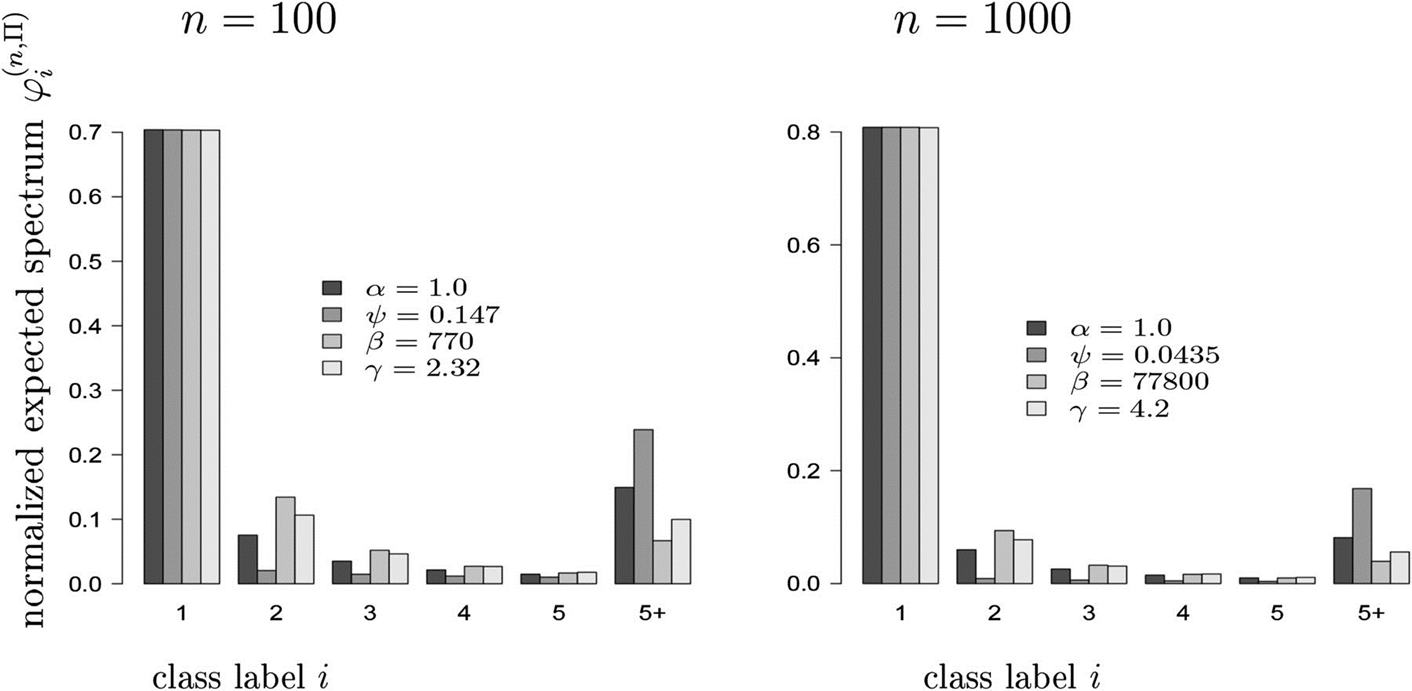
\includegraphics[width=\linewidth]{example-figure}
\caption{Example figure from \url{10.1534/genetics.114.173807}. Please include your figures in the manuscript for the review process. You can upload figures to Overleaf via the Project menu. Upon acceptance, we'll ask for your figure files to be uploaded in any of the following formats: TIFF (.tiff), JPEG (.jpg), Microsoft PowerPoint (.ppt), EPS (.eps), or Adobe Illustrator (.ai).  Images should be a minimum of 300 dpi in resolution and 500 dpi minimum if line art images.  RGB, CMYK, and Grayscale are all acceptable. Halftones should be high contrast with sharp detail, because some loss of detail and contrast is inevitable in the production process. Figures should be 10-20 cm in width and 1-25 cm in height. Graph axes must be exactly perpendicular and all lines of equal density.
Label multiple figure parts with A, B, etc. in bolded type, and use Arrows and numbers to draw attention to areas you want to highlight. Legends should start with a brief title and should be a self-contained description of the content of the figure that provides enough detail to fully understand the data presented. All conventional symbols used to indicate figure data points are available for typesetting; unconventional symbols should not be used. Italicize all mathematical variables (both in the figure legend and figure) , genotypes, and additional symbols that are normally italicized.  
}%
\label{fig:spectrum}
\end{figure}

\subsection{Sample Video}

Figure \ref{video:spectrum} shows how to include a video in your manuscript.

\begin{figure}[htbp]
\centering
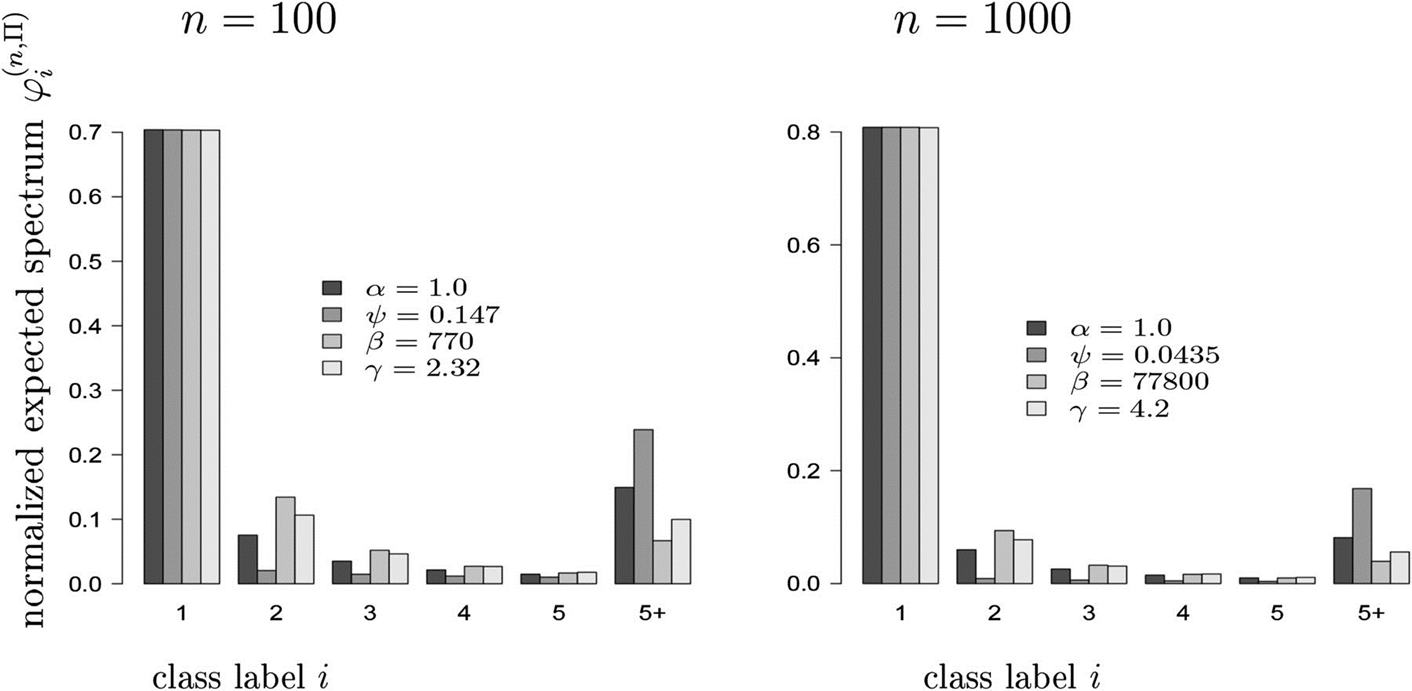
\includegraphics[width=\linewidth]{example-figure}
\caption{Example movie (the figure file above is used as a placeholder for this example). \textit{GENETICS} supports video and movie files that can be linked from any portion of the article - including the abstract. Acceptable formats include .asf, avi, .wav, and all types of Windows Media files.   
}%
\label{video:spectrum}
\end{figure}


\subsection{Sample Table}

Table \ref{tab:shape-functions} shows an example table. Avoid shading, color type, line drawings, graphics, or other illustrations within tables. Use tables for data only; present drawings, graphics, and illustrations as separate figures. Histograms should not be used to present data that can be captured easily in text or small tables, as they take up much more space.  

Tables numbers are given in Arabic numerals. Tables should not be numbered 1A, 1B, etc., but if necessary, interior parts of the table can be labeled A, B, etc. for easy reference in the text.  


\begin{table*}[htbp]
\centering
\caption{\bf Students and their grades}
\begin{tableminipage}{\textwidth}
\begin{tabularx}{\textwidth}{XXXX}
\hline
Student & Grade\footnote{This is an example of a footnote in a table. Lowercase, superscript italic letters (a, b, c, etc.) are used by default. You can also use *, **, and *** to indicate conventional levels of statistical significance, explained below the table.} & Rank & Notes \\
\hline
Alice & 82\% & 1 & Performed very well.\\
Bob & 65\% & 3 & Not up to his usual standard.\\
Charlie & 73\% & 2 & A good attempt.\\
\hline
\end{tabularx}
  \label{tab:shape-functions}
\end{tableminipage}
\end{table*}

\section{Sample Equation}

Let $X_1, X_2, \ldots, X_n$ be a sequence of independent and identically distributed random variables with $\text{E}[X_i] = \mu$ and $\text{Var}[X_i] = \sigma^2 < \infty$, and let
\begin{equation}
S_n = \frac{X_1 + X_2 + \cdots + X_n}{n}
      = \frac{1}{n}\sum_{i}^{n} X_i
\label{eq:refname1}
\end{equation}
denote their mean. Then as $n$ approaches infinity, the random variables $\sqrt{n}(S_n - \mu)$ converge in distribution to a normal $\mathcal{N}(0, \sigma^2)$.

\bibliography{example-bibliography}

\end{document}